\documentclass{beamer}

\usepackage[utf8]{inputenc}
\usepackage[T1]{fontenc}
\usepackage[english]{babel}
\usepackage{setspace}
\usepackage{color}
\usepackage{listings}
\usepackage{pgf-pie}

\usetheme[progressbar=frametitle]{metropolis}
\setbeamertemplate{frame numbering}[fraction]
\useoutertheme{metropolis}
\useinnertheme{metropolis}
\usefonttheme{metropolis}
\usecolortheme{spruce}
\setbeamercolor{background canvas}{bg=white}

\title[Micronaut]{Introduction to Micronaut Framework}
\subtitle{A modern, JVM-based, full-stack framework for building modular, easily testable microservice and serverless applications.}
\author{\texorpdfstring{Albert Attard\newline\url{albert.attard@thoughtworks.com}}{Albert Attard}}
\institute{\large \href{https://thoughtworks.com}{\textbf{ThoughtWorks}.com}}
\date{}

\begin{document}
  \metroset{block=fill}

  \begin{frame}
    \titlepage
  \end{frame}

  \begin{frame}[t]{Micronaut}
    \textbf{What is Micronaut?}\\[6pt]
    Micronaut is a framework based on the JVM that enables fast development of low memory footprint application.

    This makes it a good candidate for building microservices and serverless applications.
  \end{frame}

  \begin{frame}[t]{Another Framework?}
    \textbf{Spring Boot} dominates the market, according to \href{https://www.jrebel.com/sites/rebel/files/pdfs/ebook-jrebel-java-productivity-report.pdf}{JRebel's 2020 Java Developer Productivity Report}

    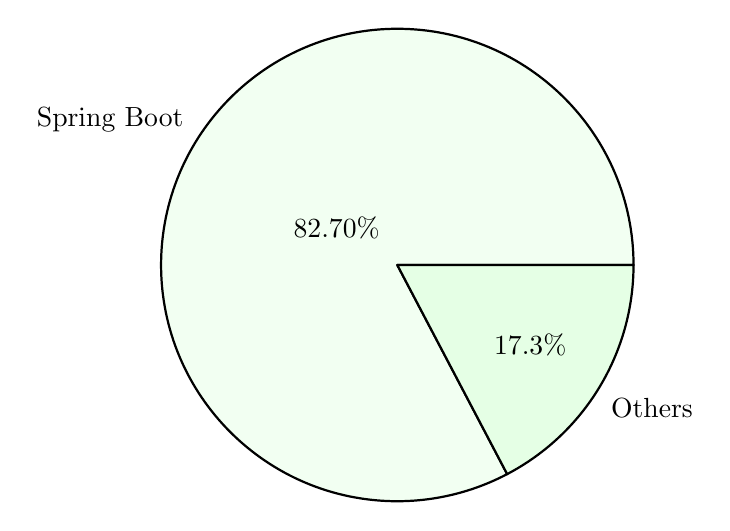
\begin{tikzpicture}
      \pie [rotate = 0, color={green!5, green!10}]
      {82.70/Spring Boot,
      17.3/Others}
    \end{tikzpicture}

  \end{frame}

  \begin{frame}[t]{using Blocks}
    \begin{block}{Micronaut}
      \textbf{Micronaut} is a modern, JVM-based, full-stack framework for building modular, easily testable microservice and serverless applications
    \end{block}
  \end{frame}

  \begin{frame}[t,fragile]{Code Example}
    Example
    \begin{lstlisting}[language=Java]
// this is a simple code listing
println("hello kotlin from latex")
    \end{lstlisting}
  \end{frame}
\end{document}
